\documentclass[a5paper, 12pt, twoside]{scrartcl}

\usepackage[europeanresistors]{circuitikz}


\usepackage{scrlayer-scrpage, siunitx, mystyle}

\usepackage[compact]{titlesec}
\titlespacing{\section}{0pt}{0ex}{0ex}
\titlespacing{\subsection}{0pt}{1ex}{0ex}
\titlespacing{\subsubsection}{0pt}{0.5ex}{0ex}
\setlength{\parskip}{0.3cm}

\graphicspath{{./Grafiken/}}

\clearpairofpagestyles{}

\setkomafont{pageheadfoot}{\sffamily\footnotesize}
\setkomafont{pagination}{}

\ohead{Seite~\pagemark}
\ihead{Emil Slomka, Tim Hilt}

\KOMAoptions{
  headsepline=true,
}

\begin{document}

\newgeometry{left=1cm, right=1cm, top=2cm, bottom=1cm}
\begin{center}
  \usekomafont{disposition}\huge Elektronik Formelsammlung
\end{center}

\section{Grundlagen und Wiederholung}

\begin{minipage}[t]{.48\textwidth}
  \mybfcol{Dezimalpräfixe}
  
  {\centering
    \begin{tabular}{lll}
      \(n\) & Nano & \(\cdot 10^{-9}\)\\
      \(\mu\) & Micro & \(\cdot 10^{-6}\)\\
      \(m\) & Milli & \(\cdot 10^{-3}\)\\
      \(K\) & Kilo & \(\cdot 10^3\)\\
      \(M\) & Mega & \(\cdot 10^6\)\\
      \(G\) & Giga & \(\cdot 10^9\)
    \end{tabular}\par
  }
  \vspace{1em}
  \mybfcol{Übertragungsfunktion}
  \[\frac{U_a}{U_e} = \frac{\text{Widerstände parallel zum Ausgang}}{\text{Widerstände parallel zum Eingang}}\]
  \mybfcol{Widerstände parallel zueinander}
  \[R_1 || R_2 = \frac{R_1 \cdot R_2}{R_1 + R_2}\]
\end{minipage}\hfill\vline\hfill%
\begin{minipage}[t]{.48\textwidth}
  \mybfcol{Spannungsquelle in Stromquelle}

  \begin{circuitikz}
    \draw (0,0) -- (3,0) to [R, l=\(R_a\)] (6,0) to [open, o-o] (6,-2.5) -- (0,-2.5) to [european current source, l=\(I_e\)] (0,0);
    \draw (3,0) to [R, l=\(R_i\), *-*] (3,-2.5);
  \end{circuitikz}
  \begin{circuitikz}
    \draw (0,0) to [R, l=\(R_i\)] (3,0) to [R, l=\(R_a\)] (6,0) to [open, o-o] (6,-2.5) -- (0,-2.5) to [european voltage source, l=\(U_e\)] (0,0);
  \end{circuitikz}

  mit
  \[U_e = I_e \cdot R_i\]
\end{minipage}

\section{Kondensator und Zeitkonstanten}

Zeitkonstante \(\tau\) beim \mybfcol{Kondensator}: \dotfill \(\tau = R \cdot C\)

Zeitkonstante \(\tau\) bei der \mybfcol{Spule}: \dotfill \(\tau = \frac{L}{R}\)

Beziehung zwischen zufließender bzw.\ abfließender Ladung und Spannung:
\[i(t) = \frac{dQ}{dt} = C \cdot \frac{du(t)}{dt} \Rightarrow u(t) = \frac{1}{C} \cdot \int i(t)\ dt\]
\mytextcol{\(\rightarrow\) Kondensator integriert den Strom auf!}

Energie im Kondensator:\dotfill\(W = \frac{1}{2} \cdot C \cdot U^2\)

\begin{figure}[H]
  \centering
  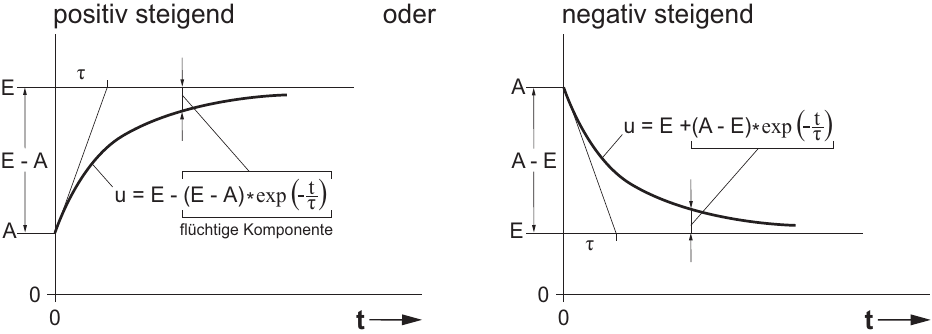
\includegraphics[width=.7\textwidth]{LadekurveKondensator}
  \caption{Ladekurven Kondensator \mybfcol{Achtung: \(t = \Delta t = t_1 - t_0\)}}
\end{figure}

\begin{center}
  \begin{tabular}{ll}
    \toprule
    Wenn Ladung von \SI{0}{\volt} nach \(U_e\): & \(U_C = U_e \cdot (1 - e^{-\frac{t}{\tau}})\)\\
    Wenn Entladung von \(U_C\) nach \SI{0}{\volt} & \(U_a = U_C \cdot e^{-\frac{t}{\tau}}\)\\
    \bottomrule
  \end{tabular}
\end{center}

\textbf{Zum Zeichnen im Zeitbereich:} Arbeitsgerade von Anfangsspannung zur Endspannung zeichnen, mit \(t = \tau\)

\mybfcol{Achtung: Immer alle Widerstände parallel und in Reihe zum Kondensator berücksichtigen und Übertragungsfunktion für Ladeziel verwenden!}

\begin{table}[H]
  \centering
  \begin{tabular}{cc}
    \toprule
    \(t=\tau\) & \(\approx 63\%\) von\ \(|A-E|\)\\
    \(t=2\tau\) & \(\approx 86\%\) von\ \(|A-E|\)\\
    \(t=5\tau\) & \(\approx 99\%\) von\ \(|A-E|\)\\
    \bottomrule
  \end{tabular}
\end{table}

\section{Dioden}

\begin{minipage}{.69\linewidth}
  \mybfcol{Strom durch Diode}\dotfill\(I_D = I_{S0} \cdot \left( e^{\frac{U_D}{mU_T}}-1 \right)\)\\[1em]
  \mybfcol{Verlustleistung in einer Diode}\dotfill\(P = U_D + I_{D\text{max}}\)\\[1em]
  \mybfcol{Mittlere Verlustleistung in einer Diode}\dotfill\(\frac{1}{T} \int_0^T U_D \cdot I_{D\text{max}}\ dt\)\\[1em]
  \mybfcol{thermischer Widerstand}\dotfill\(R_{\text{th}} = \frac{\Delta T}{P}\)\\[1em]
  \mybfcol{temperaturbedingter Zusatzwiderstand}\dotfill\(r_{z\text{th}} = TK_U \cdot U^2_{Z0} \cdot R_{\text{th}}\)
\end{minipage}\hfill%
\begin{minipage}{.29\linewidth}
  {\centering
    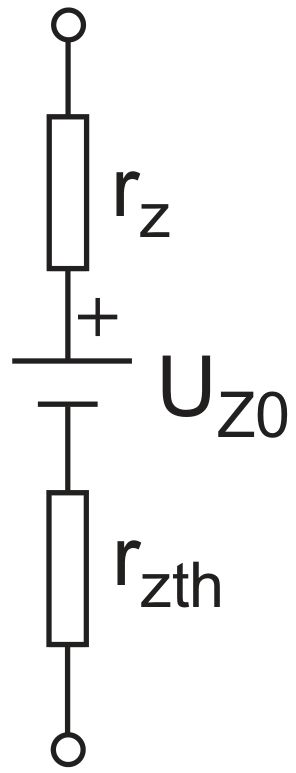
\includegraphics[width=.4\textwidth]{ESB_ZDiode}
    \captionof{figure}{Ersatzschaltbild einer Z-Diode}\par
  }
\end{minipage}

\vspace{1cm}

\mybfcol{Notiz zu Zenerdioden:} Eine Zenerdiode beginnt erst zu wirken, wenn die an der negativen Seite anliegende Spannung \textbf{größer als \(U_{Z0}\)} ist.

\clearpage

\section{Filter und Übertragungsfunktionen}

Im Fourierbereich: \(\omega = 2 \pi f\), im Laplacebereich: \(j\omega = p\)

{\centering
  \begin{tabular}{cllll}
    \toprule
    & \mybfcol{RC-Tiefpass} & \mybfcol{RC-Hochpass} & \mybfcol{RL-Tiefpass} & \mybfcol{RL-Hochpass}\\
    \midrule
    \mybfcol{Übertragungsfunktion} \(\frac{U_a}{U_e} = H(j\omega)\) & \(\frac{1}{1 + j\omega R C}\) & \(\frac{j\omega RC}{1 + j\omega RC}\) & \(\frac{R}{R + j \omega L}\)& \(\frac{j\omega L}{R + j \omega L}\) \\[1em]
    \mybfcol{Grenzfrequenz} \(f_G / \omega_G\) & \(\frac{1}{2 \pi R C}; \frac{1}{RC}\) & \(\frac{1}{2 \pi R C}; \frac{1}{RC}\) & \(\frac{R}{2 \pi L}; \frac{R}{L}\) & \(\frac{R}{2 \pi L}; \frac{R}{L}\)\\
    \bottomrule
  \end{tabular}\par
  }
\begin{minipage}{.49\linewidth}
  {\centering
    \begin{circuitikz}
      \draw (0,0) to [R, l=\(R\)] (4,0) to [C, l_=\(C\)] (4,-2) node[rground]{};
      \draw (0,0) to [european voltage source] (0,-2) node[rground]{};
      \draw (-.5,0) to [open, v=\(U_e\)] (-.5,-2);
      \draw (4.5,0) to [open, v^=\(U_a\)] (4.5,-2);
    \end{circuitikz}
    \captionof{figure}{RC-Tiefpass}\par
  }
  {\centering
    \begin{circuitikz}
      \draw (0,0) to [L, l=\(L\)] (4,0) to [R, l_=\(R\)] (4,-2) node[rground]{};
      \draw (0,0) to [european voltage source] (0,-2) node[rground]{};
      \draw (-.5,0) to [open, v=\(U_e\)] (-.5,-2);
      \draw (4.5,0) to [open, v^=\(U_a\)] (4.5,-2);
    \end{circuitikz}
    \captionof{figure}{RL-Tiefpass}\par
  }
\end{minipage}\hfill%
\begin{minipage}{.49\linewidth}
  {\centering
    \begin{circuitikz}
      \draw (0,0) to [C, l=\(C\)] (4,0) to [R, l_=\(R\)] (4,-2) node[rground]{};
      \draw (0,0) to [european voltage source] (0,-2) node[rground]{};
      \draw (-.5,0) to [open, v=\(U_e\)] (-.5,-2);
      \draw (4.5,0) to [open, v^=\(U_a\)] (4.5,-2);
    \end{circuitikz}
    \captionof{figure}{RC-Hochpass}\par
  }
  {\centering
    \begin{circuitikz}
      \draw (0,0) to [R, l=\(R\)] (4,0) to [L, l_=\(L\)] (4,-2) node[rground]{};
      \draw (0,0) to [european voltage source] (0,-2) node[rground]{};
      \draw (-.5,0) to [open, v=\(U_e\)] (-.5,-2);
      \draw (4.5,0) to [open, v^=\(U_a\)] (4.5,-2);
    \end{circuitikz}
    \captionof{figure}{RL-Hochpass}\par
  }
\end{minipage}

\vspace{1cm}

\begin{minipage}[t]{.48\linewidth}
  \mybfcol{Dämpfung bei passiven Filtern erster Ordnung:}
  \begin{itemize}
  \item Dämpfung um einen Anfangswert im Durchlassbereich (Muss berechnet werden, indem\\ \(20 \cdot \log(|H(0)|)\) berechnet wird)
  \item Anfangswert \(- \SI{3}{\decibel}\) an der Grenzfrequenz \(f_G\), bzw.\ Anfangswert \(\cdot \frac{1}{\sqrt{2}}\)
  \item \SI{6}{\decibel} pro Oktave (doppelte Frequenz) im Sperrbereich
  \item \SI{20}{\decibel} pro Dekade (zehnfache Frequenz) im Sperrbereich
  \end{itemize}
\end{minipage}\hfill\vline\hfill%
\begin{minipage}[t]{.48\linewidth}
  \mybfcol{Konstruktion von Bode-Diagrammen:}
  \begin{enumerate}
  \item \(|H(f)|\) bestimmen
  \item \(f_G\) berechnen
  \item Werte für \(f\) in \(|H(f)|\) einsetzen (für \(f=0\) und zwei Werte im Sperrbereich) und \(20\cdot\log(|H(f)|)\) berechnen
  \item Asymptoten zeichnen
  \item Bode Diagramm zeichnen, \(f_G\) befindet sich am Schnittpunkt beider Asymptoten
  \end{enumerate}
\end{minipage}

\vspace{1cm}

\mytextcol{Phase in einem \(RC\)-Netzwerk:}\dotfill\(-\arctan(\omega RC)\)

\newpage

% --------------------- OPV ---------------------
\begin{figure}[H]
  \centering
  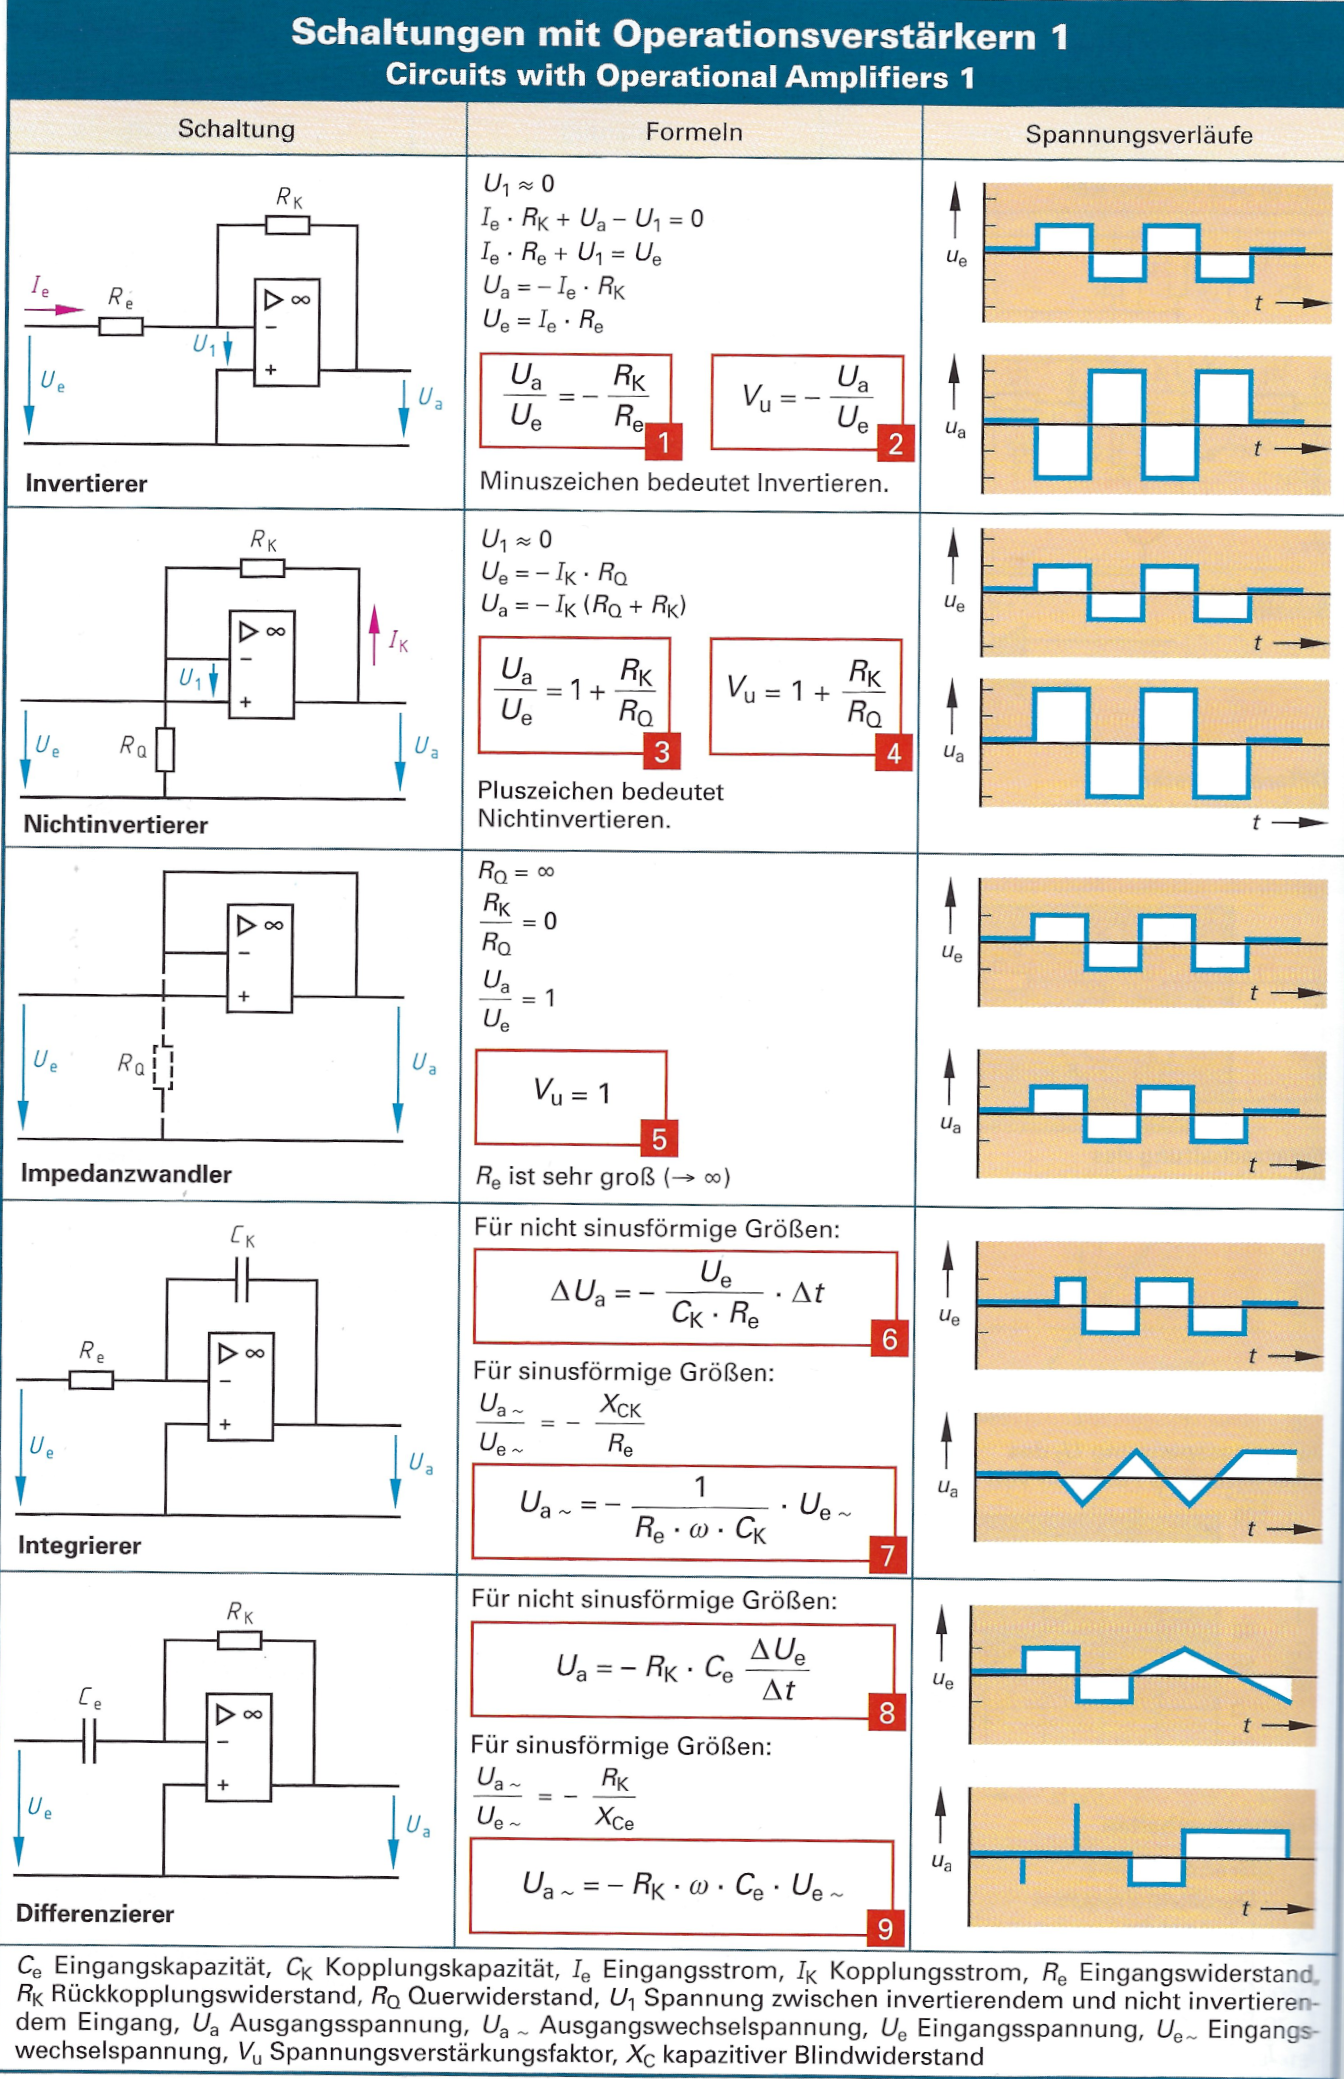
\includegraphics[width=.93\textwidth]{OPV1}
\end{figure}
\begin{figure}[H]
  \centering
  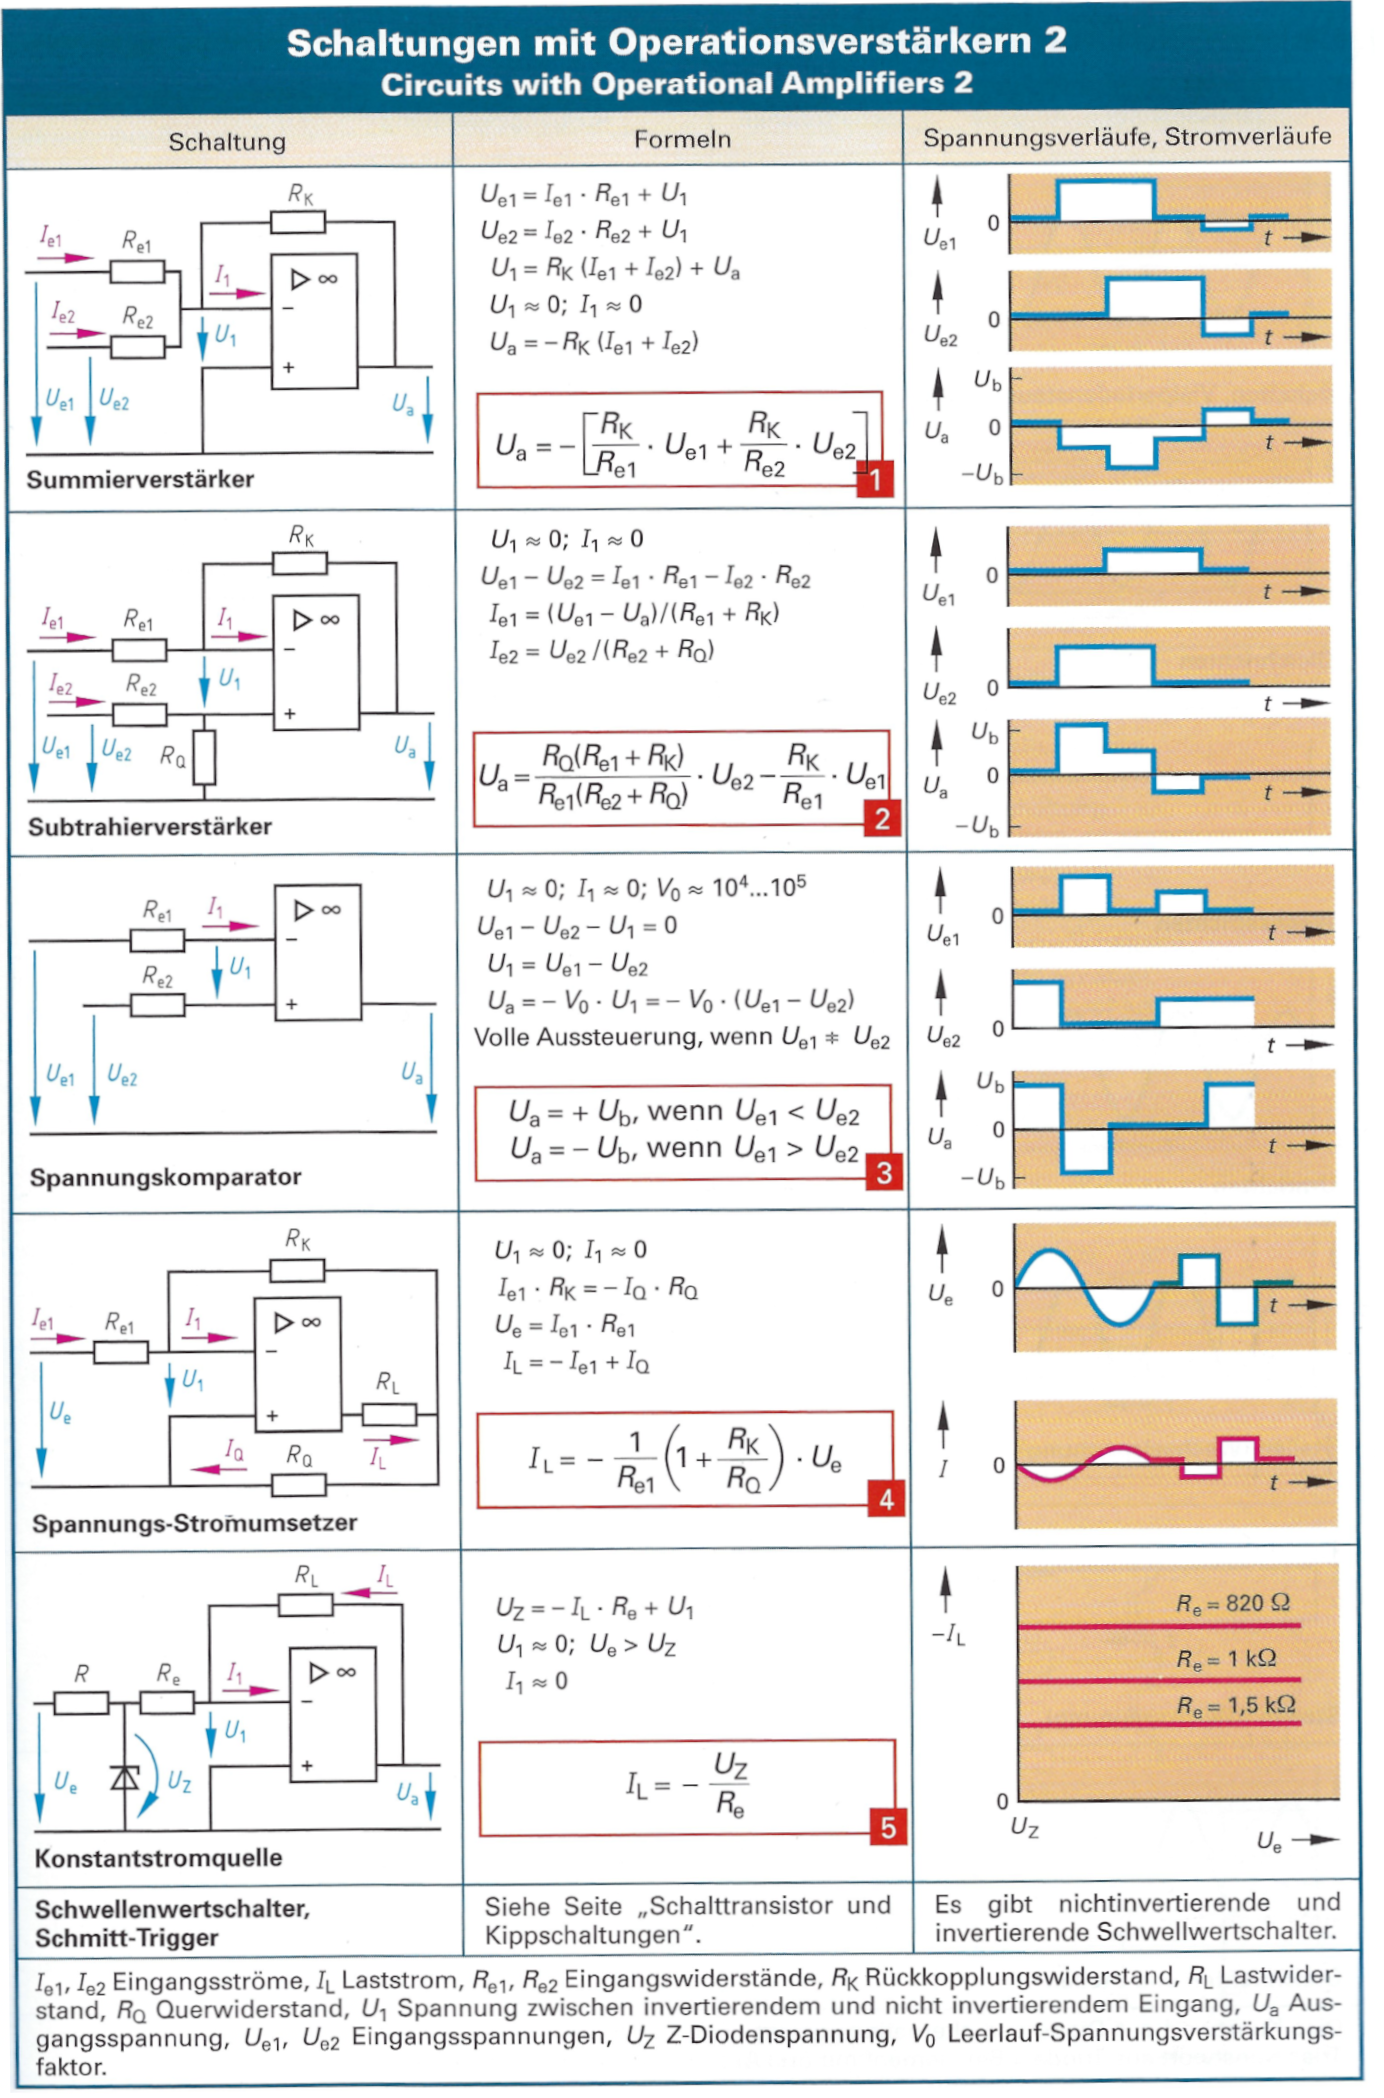
\includegraphics[width=.95\textwidth]{OPV2}
\end{figure}
% -----------------------------------------------

\section{Transistor}

\begin{minipage}{.49\linewidth}
  \begin{figure}[H]
    \centering
    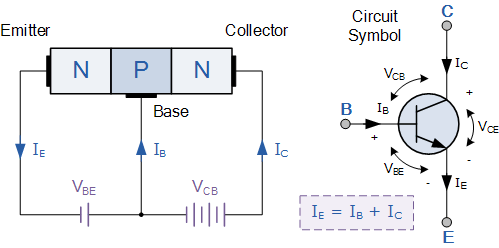
\includegraphics[width=\textwidth]{Transistor}
    \caption{Ströme im Transistor}
  \end{figure}
\end{minipage}\hfill\vline\hfill%
\begin{minipage}{.49\linewidth}
  \begin{figure}[H]
    \centering
    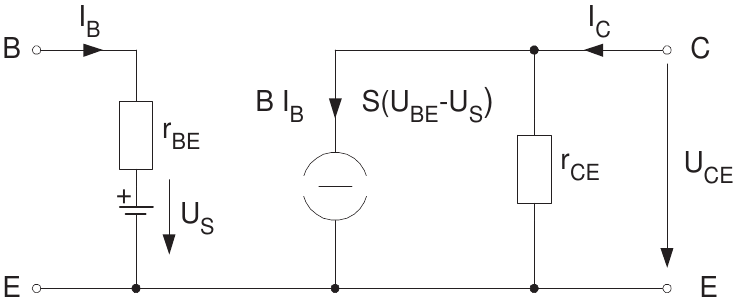
\includegraphics[width=\textwidth]{ESBTransistor}
    \caption{Ersatzschaltbild eines Bipolartransistors}
  \end{figure}
\end{minipage}

\textbf{Achtung: Beim Zeichnen des Ersatzschaltbildes wird die Spannungsquelle kurzgeschlossen! Das heißt überall wo vorher die Versorgungsspannung war ist nun GND.}

\mybfcol{Spannungsverstärkung}\dotfill\(v_u = \frac{\Delta U_a}{\Delta U_e} = -S \cdot R_C\)

\mybfcol{Stromverstärkung}\dotfill\(I_C = \beta \cdot I_B\)

\mybfcol{Verlustleistung}\dotfill\(P = U_{CE} \cdot I_C\)

\mybfcol{Steilheit}\dotfill\(S = \frac{\Delta I_C}{\Delta U_{BE}} = \frac{I_C}{U_T}\)

\mybfcol{Arbeitsgerade zeichnen}\\
\begin{enumerate}
\item Betrachte Transistor im gesperrten Zustand \(\rightarrow U_{CE} = U_B, I_C = 0\)
\item Punkt auf der \(x\)-Achse bei \(U_{CE} = U_B\) zeichnen
\item Betrachte Transistor im gesättigten Bereich \(\rightarrow U_{CE} = 0, I_C = I_{Cmax}\)
\item Berechne \(I_{Cmax}\) durch Spannungsteilerformel \(I_C = \frac{U_B}{R_C + R_E}\)
\item Punkt auf der \(y\)-Achse bei \(I_C = I_{Cmax}\) zeichnen
\item Beide Punkte durch Arbeitsgerade verbinden
\item \(U_{CE}\) im Arbeitspunkt (gegeben) kennzeichnen
\end{enumerate}

\mybfcol{Kollektorstrom \(I_C\) im Arbeitspunkt}\\
(Für gegebenes \(U_{CE0}\) im Arbeitspunkt)
\[I_{C0} = \frac{U_B - U_{CE0}}{R_C + R_E}\]

\[r_{BE} = \frac{U_T}{I_B} \qquad; U_T = \SI{26}{\milli\volt}\]

{\centering
  \includegraphics[width=\textwidth]{TransistorVerstärkerschaltung_Spannungen}
  \captionof{figure}{Spannungen an Emitterschaltung}\par%
}

\mybfcol{Für optimale Aussteuerung berühren sich \(U_C\) und \(U_E\)!}

\mybfcol{Optimale Spannungsaussteuerbarkeit}\\
Spannungen sind im Gleichgewicht
\[U_C = U_E = \frac{1}{2} \cdot U_{\text{Bat}}\]
\(U_{\text{Bat}}\) wird immer vollständig auf \(U_C\) und \(U_E\) aufgeteilt.
\[U_{\text{Bat}} = U_C + U_E\]

\end{document}


%%% Local Variables:
%%% mode: latex
%%% TeX-master: t
%%% End:
